\documentclass[bibtotoc,liststotoc,BCOR5mm,DIV12]{scrbook}

% use this declaration to set specific page margins
%\usepackage[a4paper , lmargin = {2.7cm} , rmargin = {2.9cm} , tmargin = {2.7cm} , bmargin = {4.6cm} ]{geometry}
\usepackage[a4paper]{geometry}

\usepackage[ngerman, english]{babel}
\usepackage{bibgerm}       		% german references
\usepackage[latin1]{inputenc} % german characters
\usepackage{graphicx} 				% it's recommended to use PDF images but you can use JPG or PNG as well
\usepackage{url}           		% format URLs
\usepackage{hyperref} 				% create hyperlinks
\usepackage{listings, color}	% for source code
\usepackage{subfig}						% two figures next to each other (example: figure 3a), figure 3b)
\usepackage{scrpage2}					% header and footer line

% header and footer line - no header & footer line on pages where a new chapter starts
\pagestyle{scrheadings}
\ohead{Design and Implementation of X}
\ihead{Your Name}
\ofoot[]{\thepage}
\ifoot{Diploma Thesis, TU Berlin, Fachgebiet AV, 2009}

% set path where images are stored
\graphicspath{{./img/}}

%
% der Befehl \hypenation versteht keine Sonderzeichen, also weder �
% noch "a noch \"a. W�rter die derartige Zeichen enthalten m�ssen
% direkt im Text getrennt werden, z.B. W�r\-ter
%
\hyphenation{te-le-com-muni-cation
te-le-com-muni-cation-specific
Te-le-kom-mu-ni-ka-tions-API}
 					% use this file to set explicit hyphenations (doesn't seem to work correctly)

\begin{document}
% ---------------------------------------------------------------
\frontmatter
    \thispagestyle{empty}
\begin{center}

\vspace*{1.4cm}
{\LARGE \textbf{Technische Universit�t Berlin}}

\vspace{0.5cm}

{\large Institut f�r Telekommunikationssysteme\\[1mm]}
{\large Fachgebiet Architektur der Vermittlungsknoten\\[5mm]}

Fakult�t IV\\
Franklinstrasse 28-29\\
10587 Berlin\\
http://www.av.tu-berlin.de\\

\vspace*{1cm}


\includegraphics[width=4cm]{tu_logo.jpg}

\vspace*{1.0cm}

{\LARGE Diploma Thesis}\\

\vspace{1.0cm}
{\LARGE \textbf{Hysteretic Neural Network and Trading}}\\
\vspace*{0.3cm}
% {\LARGE \textbf{of Component X}}\\
% \vspace*{1.0cm}
{\LARGE Zongxiong Chen}
\\
\vspace*{0.5cm}
Matriculation Number: 0390198\\
xx.xx.2019\\ % 	date of submission
\vspace*{1.0cm}

Supervised by\\
Prof. Dr. Thomas Magedanz\\
\vspace*{0.5cm}
Assistant Supervisor\\
Your second Supervisor
\vspace{3cm}


\end{center}

   	\thispagestyle{empty}
    \cleardoublepage
    
    \thispagestyle{empty}
\vspace*{3cm}


\begin{center}

\includegraphics[width=0.4\textwidth]{fokuspng.png}
\end{center}

\vspace*{0.2cm}

\begin{center}
FOKUS Institute\\
Kaiserin-Augusta-Allee 31\\
10589 Berlin\\
\end{center}
\vspace*{0.5cm}

\noindent This dissertation originated in cooperation with the Fraunhofer Institute for Open Communication Systems (FOKUS).

\vspace*{1cm}
\noindent 
First of all I would like to thank Prof. Dr. Thomas Magedanz at the Fraunhofer Institute FOKUS for giving me the opportunity to carry out state of the art research in this field. 
\\
\\
Special thanks to Mister X and Mister Y for their guidance. --- Some personel words... ---
\\
\\
Furthermore I would like to thank ...
    \thispagestyle{empty}
    \cleardoublepage
    
    \newpage

\thispagestyle{empty}

\begin{large}

\vspace*{6cm}

\noindent
Hereby I declare that I wrote this thesis myself with the help of no more than the mentioned literature and auxiliary means.
\vspace{2cm}

\noindent
Berlin, 01.01.2050

\vspace{3cm}

\hspace*{7cm}%
\dotfill\\
\hspace*{8.5cm}%
\textit{(Signature [your name])}

\end{large}
 
    \thispagestyle{empty}
    \cleardoublepage
    
    
    \thispagestyle{empty}
\vspace*{1.0cm}

\begin{center}
    \textbf{Abstract}
\end{center}

\vspace*{0.5cm}

\noindent
This template is intended to give an introduction of how to write diploma and master thesis at the chair 'Architektur der Vermittlungsknoten' of the Technische Universität Berlin. Please don't use the term 'Technical University' in your thesis because this is a proper name.
\\
\\
On the one hand this PDF should give a guidance to people who will soon start to write their thesis. The overall structure is explained by examples. On the other hand this text is provided as a collection of LaTeX files that can be used as a template for a new thesis. Feel free to edit the design.
\\
\\
It is highly recommended to write your thesis with LaTeX. I prefer to use Miktex in combination with TeXnicCenter (both freeware) but you can use any other LaTeX software as well. For managing the references I use the open-source tool jabref. For diagrams and graphs I tend to use MS Visio with PDF plugin. Images look much better when saved as vector images. For logos and 'external' images use JPG or PNG. In your thesis you should try to explain as much as possible with the help of images.
\\
\\
The abstract is the most important part of your thesis. Take your time to write it as good as possible. Abstract should have no more than one page. It is normal to rewrite the abstract again and again, so  probaly you won't write the final abstract before the last week of due-date. Before submitting your thesis you should give at least the abstract, the introduction and the conclusion to a native english speaker. It is likely that almost no one will read your thesis as a whole but most people will read the abstract, the introduction and the conclusion.
\\
\\
Start with some introductionary lines, followed by some words why your topic is relevant and why your solution is needed concluding with 'what I have done'. Don't use too many buzzwords. The abstract may also be read by people who are not familiar with your topic.

    \thispagestyle{empty}
    \cleardoublepage
    
    \thispagestyle{empty}
\vspace*{0.2cm}

\begin{center}
    \textbf{Zusammenfassung}
\end{center}

\vspace*{0.2cm}

\noindent 
Da die meisten Leuten an der TU deutsch als Muttersprache haben, empfiehlt es sich, das Abstract zus�tzlich auch in deutsch zu schreiben. Man kann es auch nur auf deutsch schreiben und anschlie�end einem Englisch-Muttersprachler zur �bersetzung geben.
    \thispagestyle{empty}
    
    
    \tableofcontents
    \thispagestyle{empty}
    
    \listoffigures
    \thispagestyle{empty}
    
    \listoftables
    \thispagestyle{empty}
    
% --------------------------------------------------------------

\mainmatter % comment single chapters for faster compilation

    \chapter{Introduction\label{cha:chapter1}}

This chapter should have about 4-8 pages and at least one image, describing your topic and your concept. Usually the introduction chapter is separated into subsections like 'motivation', 'objective', 'scope' and 'outline'.

\section{Motivation\label{sec:moti}}

Start describing the situation as it is today or as it has been during the last years. 'Over the last few years there has been a tendency... In recent years...'. The introduction should make people aware of the problem that you are trying to solve with your concept, respectively implementation. Don't start with 'In my thesis I will implement X'.

\section{Objective\label{sec:objective}}

What kind of problem do you adress? Which issues do you try to solve? What solution do you propose? What is your goal?
'This thesis describes an approach to combining X and Y... The aim of this work is to...'

\section{Scope\label{sec:scope}}

Here you should describe what you will do and also what you will not do. Explain a little more specific than in the objective section. 'I will implement X on the platforms Y and Z based on technology A and B.'

Conclude this subsection with an image describing 'the big picture'. How does your solution fit into a larger environment? You may also add another image with the overall structure of your component.

'Figure \ref{fig:intro} shows Component X as part of ...'
\\
\begin{figure}[htb]
  \centering
  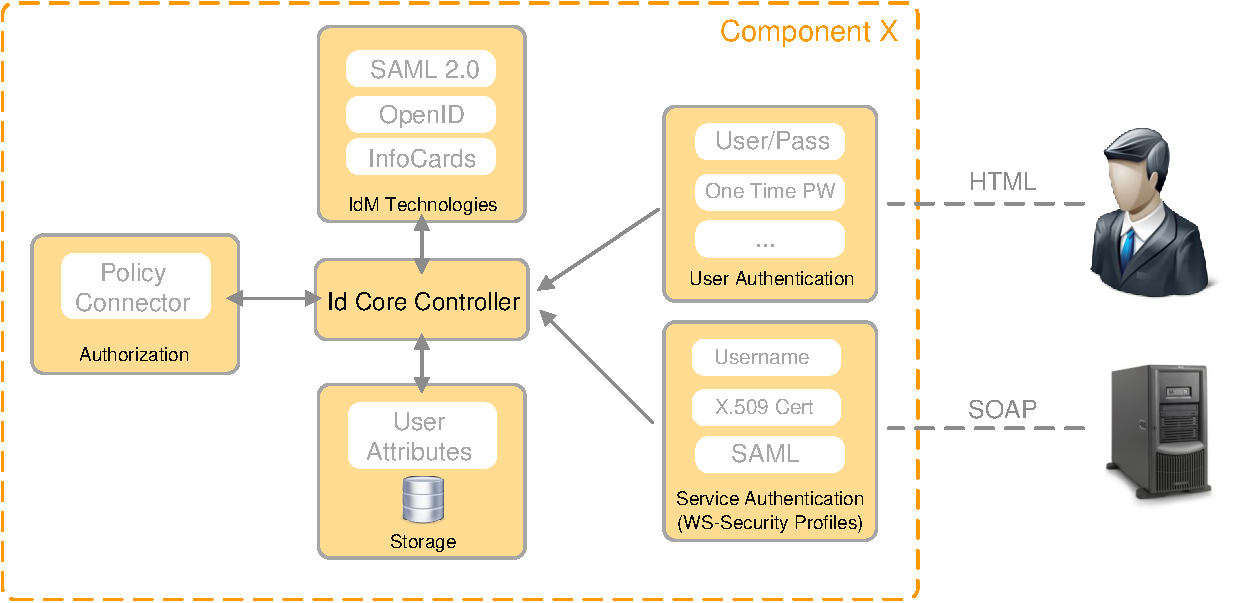
\includegraphics[width=9cm]{intro_example.pdf}\\
  \caption{Component X}\label{fig:intro}
\end{figure}

\section{Outline\label{sec:outline}}

The 'structure' or 'outline' section gives a brief introduction into the main chapters of your work. Write 2-5 lines about each chapter. Usually diploma thesis are separated into 6-8 main chapters.
\\
\\
\noindent This example thesis is separated into 7 chapters.
\\
\\
\textbf{Chapter \ref{cha:chapter2}} is usually termed 'Related Work', 'State of the Art' or 'Fundamentals'. Here you will describe relevant technologies and standards related to your topic. What did other scientists propose regarding your topic? This chapter makes about 20-30 percent of the complete thesis.
\\
\\
\textbf{Chapter \ref{cha:chapter3}} analyzes the requirements for your component. This chapter will have 5-10 pages.
\\
\\
\textbf{Chapter \ref{cha:chapter4}} is usually termed 'Concept', 'Design' or 'Model'. Here you describe your approach, give a high-level description to the architectural structure and to the single components that your solution consists of. Use structured images and UML diagrams for explanation. This chapter will have a volume of 20-30 percent of your thesis.
\\
\\
\textbf{Chapter \ref{cha:chapter5}} describes the implementation part of your work. Don't explain every code detail but emphasize important aspects of your implementation. This chapter will have a volume of 15-20 percent of your thesis.
\\
\\
\textbf{Chapter \ref{cha:chapter6}} is usually termed 'Evaluation' or 'Validation'. How did you test it? In which environment? How does it scale? Measurements, tests, screenshots. This chapter will have a volume of 10-15 percent of your thesis.
\\
\\
\textbf{Chapter \ref{cha:chapter7}} summarizes the thesis, describes the problems that occurred and gives an outlook about future work. Should have about 4-6 pages.

    \chapter{Fundamentals and Related Work\label{cha:chapter2}}

This section is intended to give an introduction about relevant terms, technologies and standards in the field of X. You do not have to explain common technologies such as HTML or XML. 

\section{Technologies \label{sec:tech}}

This section describes relevant technologies, starting with X followed by Y, concluding with Z.

\subsection{Technology A\label{sec:aaa}}

It's always a good idea to explain a technology or a system with a citation of a prominent source, such as a widely accepted technical book or a famous person or organization. 

Exmple: Tim-Berners-Lee describes the ''WorldWideWeb'' as follows:
\\
\textit{''The WorldWideWeb (W3) is a wide-area hypermedia information retrieval initiative aiming to give universal access to a large universe of documents.''} \cite{timwww}
\\
\\
You can also cite different claims about the same term.
\\
According to Bill Gates \textit{''Windows 7 is the best operating system that has ever been released''} \cite{billgates} (no real quote)
In opposite Steve Jobs claims Leopard to be \textit{''the one and only operating system''} \cite{stevejobs}

If the topic you are talking about can be grouped into different categories you can start with a classification.
Example: According to Tim Berners-Lee XYZ can be classified into three different groups, depending on foobar \cite{timwww}:
	\begin{itemize}
		\item Mobile X
				\vspace{-0.1in} 
		\item Fixed X
				\vspace{-0.1in} 
		\item Combined X
 	\end{itemize}

\subsection{Technology B\label{sec:bbb}}

For internal references use the 'ref' tag of LaTeX. Technology B is similar to Technology A as described in section \ref{sec:aaa}.

\newpage

\subsection{Comparison of Technologies\label{sec:comp}}

\begin{table}[htb]
\centering
\begin{tabular}[t]{|l|l|l|l|}
\hline
Name & Vendor & Release Year & Platform \\
\hline
\hline
A & Microsoft & 2000 & Windows \\
\hline
B & Yahoo! & 2003 & Windows, Mac OS \\
\hline
C & Apple & 2005 & Mac OS \\
\hline
D & Google & 2005 & Windows, Linux, Mac OS \\
\hline
\end{tabular}
\caption{Comparison of technologies}
\label{tab:enghistory}
\end{table}

\section{Standardization \label{sec:standard}}

This sections outlines standardization approaches regarding X.

\subsection{Internet Engineering Task Force\label{sec:itu}}

The IETF defines SIP as '...' \cite{rfcsip}

\subsection{International Telecommunication Union\label{sec:itu}}

Lorem Ipsum...

\subsection{3GPP\label{sec:3gpp}}

Lorem Ipsum...

\subsection{Open Mobile Alliance\label{sec:oma}}

Lorem Ipsum...

\section{Concurrent Approaches \label{sec:summ}}

There are lots of people who tried to implement Component X. The most relevant are ...
    \chapter{Methodology\label{cha:chapter3}}
This section determines the requirements necessary for X. This includes the functional aspects, namely Y and Z, and the non functional aspects such as A and B.

\section{Overview\label{sec:chapter3:overview}}

% In this chapter you will describe the requirements for your component. Try to group the requirements into subsections such as 'technical requirements', 'functional requirements', 'social requirements' or something like this. If your component consist of different partial components you can also group the requirements for the corresponding parts.

% Explain the source of the requirements.

% Example: The requirements for an X have been wide
% ly investigated by Organization Y.

In his paper about Z, Mister X outlines the following requirements for a Component X.

% \section{Technical Requirements\label{sec:techreq}}

% The following subsection outlines the technical requirements to Component X.

% \subsection{Sub-component A\label{sec:reqsuba}}

% \textbf{Interoperability}
% \\
% Lorem Ipsum...
% \\
% \\
% \textbf{Scalability}
% \\
% Lorem Ipsum...

% \subsection{Sub-component B\label{sec:reqsubb}}

% Lorem Ipsum...

% \section{Social Requirements\label{sec:socreq}}

% Component X must compete with Y. Hence, it is required to provide an excellent usability. This includes ...

\section{Hysteretic neural networks\label{sec:chapter3:hnn}}
\subsection{Play and Prandtl-Ishlinskii networkds\label{sec:chapter3:play-and-pi-networks}}
\\
Consider $K > 0$ play operators. Each of them maps an initial state $p_{0}^{k} \in \mathbb{R} $ and an input sequence $x_1, x_2, \ldots$ to an output sequence $p_{1}^{k}, p_{2}^{k}, \ldots \ $, i.e.,

% \begin{equation}\label{eqn:input_to_op_output_mapping}
\begin{equation*}
  p_{0}^{k}, (x_1, x_2, \ldots) \mapsto (p_{1}^{k}, p_{2}^{k}, \ldots), k = 1, \ldots, K
\end{equation*}

The $k$th play operator is given by:

\begin{equation}\label{\eqn:chapter3:play-operator}
  p_{n}^{k} = G(x_{n}, p_{n-1}^{k}, w^{k}) := p_{n-1}^{k} + \Phi(w^{k} x_{n} - p_{n-1}^{k}), n = 1, 2, \ldots
\end{equation}

where $w^{k}$ are parameters and

\begin{equation}\label{\eqn:chapter3:phi}
  \begin{aligned*}
    \Phi(x) =
    \begin{cases}
      x - \frac{1}{2}, & x > \frac{1}{2} \\
      0,               & -\frac{1}{2} <= x <= \frac{1}{2} \\
      x + \frac{1}{2}, & x < \frac{1}{2}
    \end{cases}
  \end{aligned*}
\end{equation}

See Fig. \ref{fig:chapter3:phi}

\begin{figure}[htb]
  \centering
  \resizebox{8cm}{!}{\documentclass{standalone}
\usepackage{tikz}
\begin{document}
\begin{tikzpicture}
% horizontal axis
\draw[->] (0,0) -- (6,0) node[anchor=north] {$f/f_N$};
% labels
\draw	(0,0) node[anchor=north] {0}
		(2,0) node[anchor=north] {1}
		(4,0) node[anchor=north] {2};
% ranges
\draw	(1,3.5) node{{\scriptsize Constant flux}}
		(4,3.5) node{{\scriptsize Field weakening}};

% vertical axis
\draw[->] (0,0) -- (0,4) node[anchor=east] {$U_s,\varPsi_s$};
% nominal speed
\draw[dotted] (2,0) -- (2,4);

% Us
\draw[thick] (0,0) -- (2,2) -- (6,2);
\draw (1,1.5) node {$U_s$}; %label

% Psis
\draw[thick,dashed] (0,3) -- (2,3) parabola[bend at end] (6,1);
\draw (2.5,3) node {$\varPsi_s$}; %label

\end{tikzpicture}
\end{document}
}
  \caption{$\Phi(x)$}\label{fig:chapter3:phi}
\end{figure}

It can be represented as a recurrent neural network, see Fig. \ref{fig:chapter3:phi}. Note that in such a form the network is not feed-forward.
One can unfold it to make it feed-forwaard, see Fig. \ref{fig:chapater3:play-operator}

*Definition 1.1.* We call this network a \textsl{play network}. If there are \textsl{m} elements in the sequence ${x_n}$, we say the unfolded network is \textsl{m-unfolded}

For example, the network in Fig. \ref{fig:chapter3:unfolded-nn} is 2-unfolded.


\subsection{Play layers and Prandtl-Ishlinskii networkds\label{sec:chapter3:play-layers-and-pi-networks}}

\subsection{Training a PI network\label{sec:chapter3:training-pi-network}}
Assume we are given an input sequence $x_1, x_2, \ldots, x_N$ and an output sequence $q_1, q_2, \ldots, q_N$. We perform the following steps in cycle until convergence.

\begin{enumerate}
\item Preparing initial states for the $m$-unfolded network: Fix a vector of initial states $P_0$ and all the weights (denoted by $W$). For each $k=1, \ldots, K$, we calculate recursively $p_{1}^{k}, p_{2}^{k}, \ldots, p_{N}^{k}$ by formula \ref{eqn:chapter3:play-operator}. We denote the corresponding (intermediate) states of the \textbf{PI} operator by
  \begin{equation*}
    P_n = (p_{n}^{1}, \ldots, p_{n}^{K}), n = 1, \ldots, N.
  \end{equation*}
\item Preparing inputs for the $m$-unfolded network: We fix $m$ and group the input sequence into $m$-tuples:
  \begin{equation*}
    \mathbf{x_1} := (x_1, \ldots, x_m), \quad \mathbf{x_2} := (x_2, \ldots, x_{m+1}), \quad \ldots,
  \end{equation*}
  which gives $M := N-m$ tuples $\mathbf{x_1}, \ldots, \mathbf{x_M}$. Next we form a new set of inputs for the $m$-unfolded network, attaching the vectors of intermediate states:
  \begin{equation*}
    \mathbf{y_1} := (P_0, \mathbf{x_1}), \quad \mathbf{y_2} := (P_1, \mathbf{x_2}), \quad \ldots,
  \end{equation*}

\item Training the $m$-unfoled network: We train by stochstic gradient descent the feed-forward $m$-unfolded \textbf{PI} network
  \begin{equation*}
    \mathbb{R}^{K} \times \mathbb{R}^{m} \ni \mathbf{y} \mapsto F_{m}(\mathbf{y}) \in \mathbb{R}^m
  \end{equation*}
  with the inputs $\mathbf{y_1}, \ldots, \mathbf{y_M}$ and the true targets $mathbf{q_1}, \ldots, mathbf{q_M}$, where
  \begin{equation*}
    \begin{aligned*}
      \mathbf{q_1} = (q_1, \ldots, \q_m), \quad \mathbf{q_2} = (q_2, \ldots, q_{m+1}), \quad \ldots
    \end{aligned*}
  \end{equation*}

\item We update the initial state $P_0$:
  \begin{equation*}
    P_{0}^{new} := P_{0} - \nabla_{P_0} (F_m(P_0, \mathbf{x_1}) - \mathbf{q_1})^2
  \end{equation*}
\end{enumerate}

\subsection{General hysteretic networks\label{sec:chapter3:general-hysteretic-networks}}
A general network may consist of several play layers (and perhaps standard layers). We can such a network \textsl{hysteretic}, and denote
\begin{equation*}
  p_n = F(X_n, W)
\end{equation*}
where $X_n = (x_1, \ldots, x_n)$ and $w$ is a vector of all weights of the network.

    \chapter{Concept\label{cha:chapter4}}
This chapter introduces the architectural design of Component X. The component consists of subcomponent A, B and C.

In the end of this chapter you should write a specification for your solution, including interfaces, protocols and parameters.

\section{Sub-component A\label{sec:conceptsuba}}
The concept chapter provides a high-level explanation of your solution. Try to explain the overall structure with a picture. You can also use UML sequence diagrams for explanation.

Figure \ref{fig:aliceandbob} illustrates the situation between Alice and Bob. (sequence diagram from www.websequencediagrams.com)

\begin{figure}[htb]
  \centering
  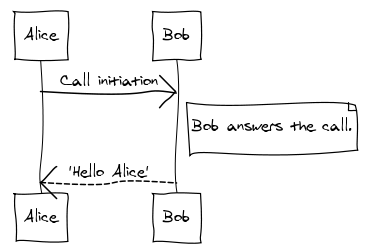
\includegraphics[width=9cm]{uml_seq_example.png}\\
  \caption{Alice and Bob}
  \label{fig:aliceandbob}
\end{figure}

\section{Sub-component B\label{sec:conceptsubb}}

Lorem Ipsum...

\section{Proposed API\label{sec:conceptsubb}}

Lorem Ipsum...

\section{Layer X\label{sec:conceptlayerx}}

Lorem Ipsum...

\section{Interworking of X and Y\label{sec:conceptinter}}

Lorem Ipsum...

\section{Interface Specification\label{sec:intspec}}

Lorem Ipsum...


    \chapter{Implementation\label{cha:chapter5}}

This chapter describes the implementation of component X. Three systems were chosen as reference implementations: a desktop version for Windows and Linux PCs, a Windows Mobile version for Pocket PCs and a mobile version based on Android. 

\section{Environment\label{sec:env}}
The following software, respectively operating systems, were used for the implementation:

\begin{itemize}
		\item Windows XP and Ubuntu 6
		\vspace{-0.1in} 
		\item Java Development Kit (JDK) 6 Update 10 
		\vspace{-0.1in} 
		\item Eclipse Ganymede 3.4
		\vspace{-0.1in} 
		\item Standard Widget Toolkit 3.4
\end{itemize}

\section{Project Structure\label{sec:projectstructure}}

The implementation is seperated into 2 distinguished eclipse projects as depicted in figure \ref{fig:projects}.

\begin{figure}[htb]
  \centering
  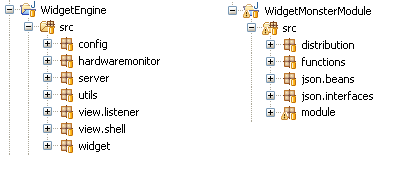
\includegraphics[width=10cm]{screenshot_2_projects}
  \caption{Project Structure}
  \label{fig:projects}
\end{figure}

\noindent
The following listing briefly describes the single packages of both projects in alphabetical order to give an overview of the implementation:
\\
\\
\textbf{config} 
\\
Lorem Ipsum...
\\
\\
\textbf{server} 
\\
Lorem Ipsum...
\\
\\
\textbf{utils} 
\\
Lorem Ipsum...

\section{Important Implementation Aspects\label{sec:gui}}

Do not explain every class in detail. Give a short introduction about the modules or the eclipse projects. If you want to explain relevant code snippets use the 'lstlisting' tag of LaTeX. Put only short snippets into your thesis. Long listing should be part of the annex.

\lstset{caption=JSON String Code Snippet,label=jsonstring,showstringspaces=false}
\begin{lstlisting}
{
	id: 1,
	method: "myInstance.getGroup",
	params: ["Teammates", 2, true]
}

{
	id: 2,
	result: [
		  "groupDesc":"These are my teammates",
		  {
			"javaClass":"src.package.MemberClass",
			"memberName": "Bob",      
		  }
		]
}\end{lstlisting}

You can also compare different approaches. Example: Since the implementation based on X failed I choosed to implement the same aspect based on Y. The new approach resulted in a much faster ...

\section{Graphical User Interface\label{sec:gui}}

Lorem Ipsum...

\section{Documentation\label{sec:docu}}

Lorem Ipsum...



    \chapter{Evaluation\label{cha:chapter6}}

In this chapter the implementation of Component X is evaluated. An example instance was created for every service. The following chapter validates the component implemented in the previous chapter against the requirements.
\\
\\
Put some screenshots in this section! Map the requirements with your proposed solution. Compare it with related work. Why is your solution better than a concurrent approach from another organization?

\section{Test Environment\label{sec:testenvir}}

Fraunhofer Institute FOKUS' Open IMS Playground was used as a test environment for the telecommunication services. The IMS Playground ...

\section{Scalability\label{sec:scal}}

Lorem Ipsum

\section{Usability\label{sec:usab}}

Lorem Ipsum

\section{Performance Measurements\label{sec:performance}}

Lorem Ipsum
    \chapter{Conclusion\label{cha:chapter7}}
The final chapter summarizes the thesis. The first subsection outlines the main ideas behind Component X and recapitulates the work steps. Issues that remained unsolved are then described. Finally the potential of the proposed solution and future work is surveyed in an outlook.

\section{Summary\label{sec:summary}}

Explain what you did during the last 6 month on 1 or 2 pages!
\\
\\
\noindent The work done can be summarized into the following work steps

\begin{itemize}
		\item Analysis of available technologies
		\vspace{-0.11in} 
		\item Selection of 3 relevant services for implementation
		\vspace{-0.11in} 
		\item Design and implementation of X on Windows
		\vspace{-0.11in} 
		\item Design and implementation of X on mobile devices
		\vspace{-0.11in} 
		\item Documentation based on X
		\vspace{-0.11in} 
		\item Evaluation of the proposed solution
\end{itemize}

\section{Dissemination\label{sec:dissemination}}

Who uses your component or who will use it? Industry projects, EU projects, open source...? Is it integrated into a larger environment? Did you publish any papers?

\section{Problems Encountered\label{sec:problems}}

Summarize the main problems. How did you solve them? Why didn't you solve them?

\section{Outlook\label{sec:outlook}}

Future work will enhance Component X with new services and features that can be used ...

% ---------------------------------------------------------------
\backmatter % no page numbering from here
    \addchap{List of Acronyms}

\begin{tabbing}
spacespacespace \= space \kill
3GPP	 \> 	3rd Generation Partnership Project	 \\
AJAX	\>	Asynchronous JavaScript and XML \\
API	 \> 	Application Programming Interface	 \\
AS	\>	Application Server \\
CSCF	 \> 	Call Session Control Function	 \\
CSS	\>	Cascading Stylesheets \\
DHTML	\>	Dynamic HTML \\
DOM	\>	Document Object Model \\
FOKUS	\>	Fraunhofer Institut fuer offene Kommunikationssysteme \\
GUI	\>	Graphical User Interface \\
GPS	\>	Global Positioning System \\
GSM	\>	Global System for Mobile Communication\\
HTML	\>	Hypertext Markup Language \\
HSS	 \> 	Home Subscriber Server	 \\
HTTP	 \> 	Hypertext Transfer Protocol	 \\
I-CSCF	 \> 	Interrogating-Call Session Control Function	 \\
IETF	\>	Internet Engineering Task Force \\
IM	\>	Instant Messaging \\
IMS	 \> 	IP Multimedia Subsystem	 \\
IP	 \> 	Internet Protocol	 \\
J2ME	\>	Java Micro Edition \\
JDK	\>	Java Developer Kit \\
JRE	\>	Java Runtime Environment \\
JSON	\>	JavaScript Object Notation \\
JSR	\>	Java Specification Request \\
JVM	 \> 	Java Virtual Machine	 \\
NGN	 \> 	Next Generation Network	 \\
OMA	 \> 	Open Mobile Alliance	 \\
P-CSCF	 \> 	Proxy-Call Session Control Function	 \\
PDA	\>	Personal Digital Assistant \\
PEEM	 \> 	Policy Evaluation, Enforcement and Management	 \\
QoS	 \> 	Quality of Service	 \\
S-CSCF	 \> 	Serving-Call Session Control Function	 \\
SDK	\>	Software Developer Kit \\
SDP	\>	Session Description Protocol \\
SIP	 \> 	Session Initiation Protocol	 \\
SMS	\>	Short Message Service \\
SMSC	\> Short Message Service Center \\
SOAP	 \> 	Simple Object Access Protocol	 \\
SWF	\>	Shockwave Flash \\
SWT	\>	Standard Widget Toolkit \\
TCP	 \> 	Transmission Control Protocol	 \\
Telco API	\>	Telecommunication API \\
TLS	\>	Transport Layer Security \\
UMTS	 \> 	Universal Mobile Telecommunication System	 \\
URI	 \> 	Uniform Resource Identifier	 \\
VoIP	 \> 	Voice over Internet Protocol	 \\
W3C	 \> 	World Wide Web Consortium	 \\
WSDL	\>	Web Service Description Language \\
XCAP	 \> 	XML Configuration Access Protocol	 \\
XDMS	 \> 	XML Document Management Server	 \\
XML	 \> 	Extensible Markup Language	 \\
\end{tabbing}
\endinput

		
		% if you want to provide a glossary with explanations of important terms put it in here

    \bibliographystyle{geralpha}
    \bibliography{./bib/references}
    
    \addchap{Annex}

\begin{appendix}

\lstset{language=,caption=Sourcecode Listing,captionpos=b,
label=yahoowidgetkon,showstringspaces=false,
basicstyle={\fontfamily{pcr}\selectfont\footnotesize}}
\begin{lstlisting}
<?xml version="1.0" encoding="UTF-8"?>
<widget>
	 <debug>off</debug>
	 <window name="myWindow" title="Hello Widget" visible="true">
		 <height>120</height>
		 <width>320</width>
		 <image src="Resources/orangebg.png">
			<name>orangebg</name>
			<hOffset>0</hOffset>
			<vOffset>0</vOffset>
		</image>
		 <text>
			 <name>myText</name>
			 <data>Hello Widget</data>
			 <color>#000000</color>
			 <size>20</size>
			 <vOffset>50</vOffset>
			 <hOffset>120</hOffset>
		 </text>
	</window>
</widget>
\end{lstlisting}

\newpage


\lstset{caption=SIP request and response packet\cite{SIPBook},
captionpos=b,label=sippacket,showstringspaces=false,
basicstyle={\fontfamily{pcr}\selectfont\footnotesize}}
\begin{lstlisting}
INVITE sip:bob@network.org SIP/2.0
Via: SIP/2.0/UDP 100.101.102.103:5060;branch=z9hG4bKmp17a
Max-Forwards: 70
To: Bob <sip:bob@network.org>
From: Alice <sip:alice@ims-network.org>;tag=42
Call-ID: 10@100.101.102.103
CSeq: 1 INVITE
Subject: How are you?
Contact: <sip:xyz@network.org>
Content-Type: application/sdp
Content-Length: 159
v=0
o=alice 2890844526 2890844526 IN IP4 100.101.102.103
s=Phone Call
t=0 0
c=IN IP4 100.101.102.103
m=audio 49170 RTP/AVP 0
a=rtpmap:0 PCMU/8000

SIP/2.0 200 OK
Via: SIP/2.0/UDP proxy.network.org:5060;branch=z9hG4bK83842.1
;received=100.101.102.105
Via: SIP/2.0/UDP 100.101.102.103:5060;branch=z9hG4bKmp17a
To: Bob <sip:bob@network.org>;tag=314159
From: Alice <sip:alice@network.org>;tag=42
Call-ID: 10@100.101.102.103
CSeq: 1 INVITE
Contact: <sip:foo@network.org>
Content-Type: application/sdp
Content-Length: 159
v=0
o=bob 2890844526 2890844526 IN IP4 200.201.202.203
s=Phone Call
c=IN IP4 200.201.202.203
t=0 0
m=audio 49172 RTP/AVP 0
a=rtpmap:0 PCMU/8000
\end{lstlisting}


\end{appendix}

\endinput


\end{document}
